\documentclass[12pt]{article}

\usepackage[utf8]{inputenc}
\usepackage[T1]{fontenc}
\usepackage{amsmath}
\usepackage{amssymb}
\usepackage{polski} 
\usepackage{graphicx}
\usepackage{caption}
\usepackage{placeins}
\usepackage{float}
\usepackage{geometry}

\addtolength{\textwidth}{3cm}
\addtolength{\hoffset}{-1cm}
\addtolength{\textheight}{3cm}
\addtolength{\voffset}{-1cm}

\setlength{\parindent}{0pt}
\setlength{\parskip}{1ex}

\author{Aleksandra Wichrowska, Karol Pysiak\\
\small Grupa F5}
\title{Klasyfikacja na zbiorze  Home Credit Default Risk\\
	\bigskip
\large Projekt nr 1\\
\bigskip
\large Wstęp do Uczenia Maszynowego\\
Wydział Matematyki i Nauk Informacyjnych\\
Politechnika Warszawska\\
\bigskip}


\textheight 23.2 cm

\textwidth 6.0 in

\hoffset = 0 in

\voffset = -2.4 cm

\begin{document}
	
	\maketitle
\begin{abstract}
Celem naszego projektu była klasyfikacja klientów pod względem problemów ze spłatą kredytu. Przed rozpoczęciem zaawansowanej pracy z danymi przeprowadziliśmy wstępną eksplorację danych, aby poznać z jakimi danymi dokładnie mamy doczynienia, jak są one zbudowane oraz co możemy z nich uzyskać. Następnie przeszliśmy do inżynierii cech, która pozwoliła nam wyodrębnić najważniejsze zmienne oraz stworzyć nowe, bardziej adekwatne do problemu zmienne. Dalej przeszliśmy do wybrania odpowiednich modeli klasyfikacyjnych, by na końcu dostroić parametry optymalnym modelom.
\end{abstract}
	\newpage
	
	\tableofcontents
	
	\newpage


\section{Wstępna eksploracja danych}

\subsection{Zależnosci między zbiorami danych}

Pierwszym krokiem do zrozumienia dostępnych danych było przyjrzenie się zależnosciom między poszczególnymi zbiorami danych. Prezentuje to poniższy schemat:

\begin{figure}[h!]
\centering
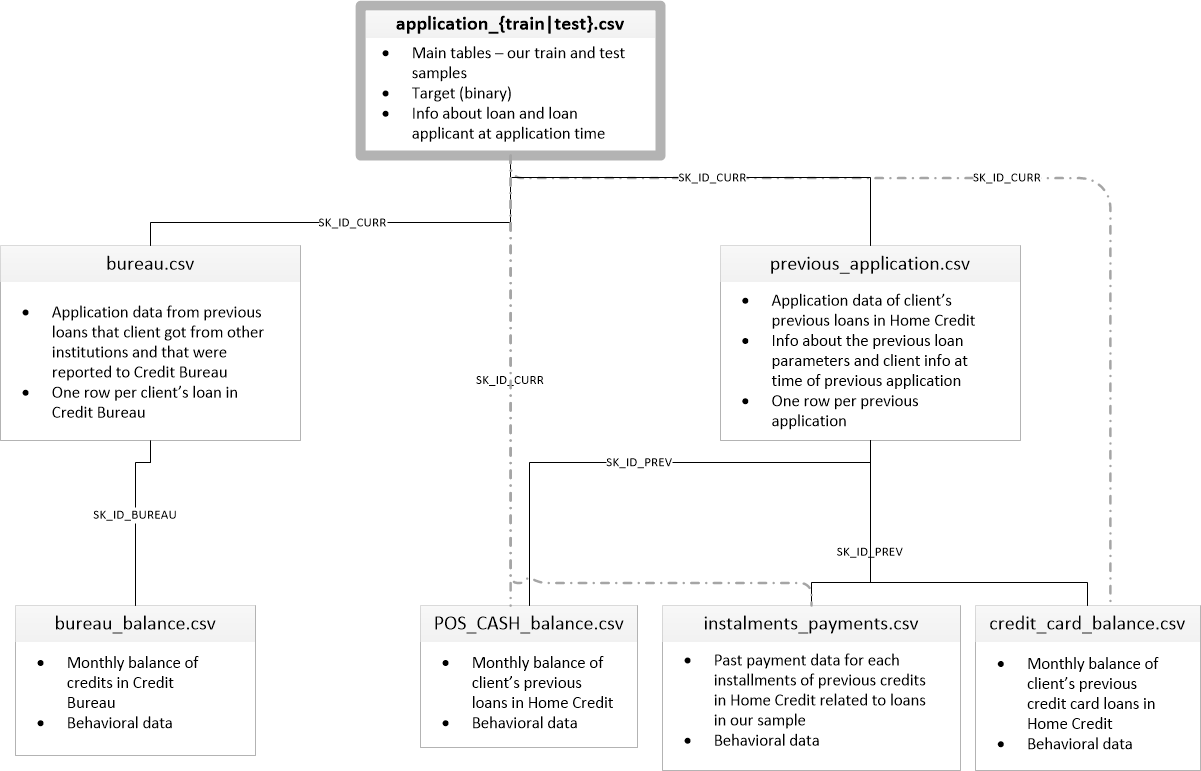
\includegraphics[scale=0.5]{zbiory.png}
\caption{Schemat zależności tabel w zbiorze danych}
\end{figure}

\subsection{Krótki opis zbiorów danych}

Zbiór $application\_train$ jest główną składową dostępnych danych. Zawiera dane o~wszystkich bieżących aplikacjach kredytowych do ''naszego banku''.

Zbiór $bureau$ zawiera informacje o poprzednich kredytach klientów  ''naszego banku'' w innych placówkach. Dodatkowo zbiór $bureau\_balance$ zawiera dane o miesięcznym bilansie kredytowym.

Zbiór $previous\_application$ zawiera w sobie informacje o poprzednich kredytach klientów w~'naszym banku'. Zależne od niego zbiory to $credit\_card\_balance$ oraz  $installments\_payments$. Dla poszczególnych kredytów zawierają one odpowiednio informacje o bilansie karty kredytowej w kolejnych miesiącach oraz o spłacanych ratach.

\subsection{Podstawowe informacje o zbiorach danych}

\FloatBarrier

\begin{table}[h]
\begin{tabular}{lcccc}

nazwa zbioru & wiersze & kolumny & kolumny numeryczne & kolumny kategoryczne \\
\hline \hline
application\_train    & 184507 & 123 & 106 & 19   \\
bureau                & 1716428 & 17 & 14 & 3  \\
bureau\_balance       & 27299925 & 3 & 2 & 1 \\
previous\_application & 1670214  & 37 & 21 &  16 \\
credit\_card          & 3840312  & 23 & 22 & 1   \\
installment\_payments & 13605401 & 8 & 8 & 0  \\
\end{tabular}
\end{table}

\FloatBarrier

\subsection{Wartosci NA}

\subsubsection{application\_train}

Sumarycznie zbiór danych zawiera około 24\% wartosci NA.

41 kolumn zawiera ponad połowę brakujących wartosci.

Poniżej fragment tabeli pokazującej, jaki procent wartości w kolumnie stanowią NA:


\begin{figure}[h!]
\centering
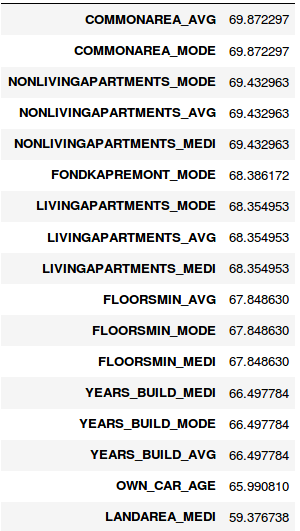
\includegraphics[scale=0.5]{NA.png}
\caption{Tabela przedstawiająca procent brakujących wartości w kolumnach $application$}
\end{figure}

\FloatBarrier

oraz wykres 


\begin{figure}[h!]
\centering
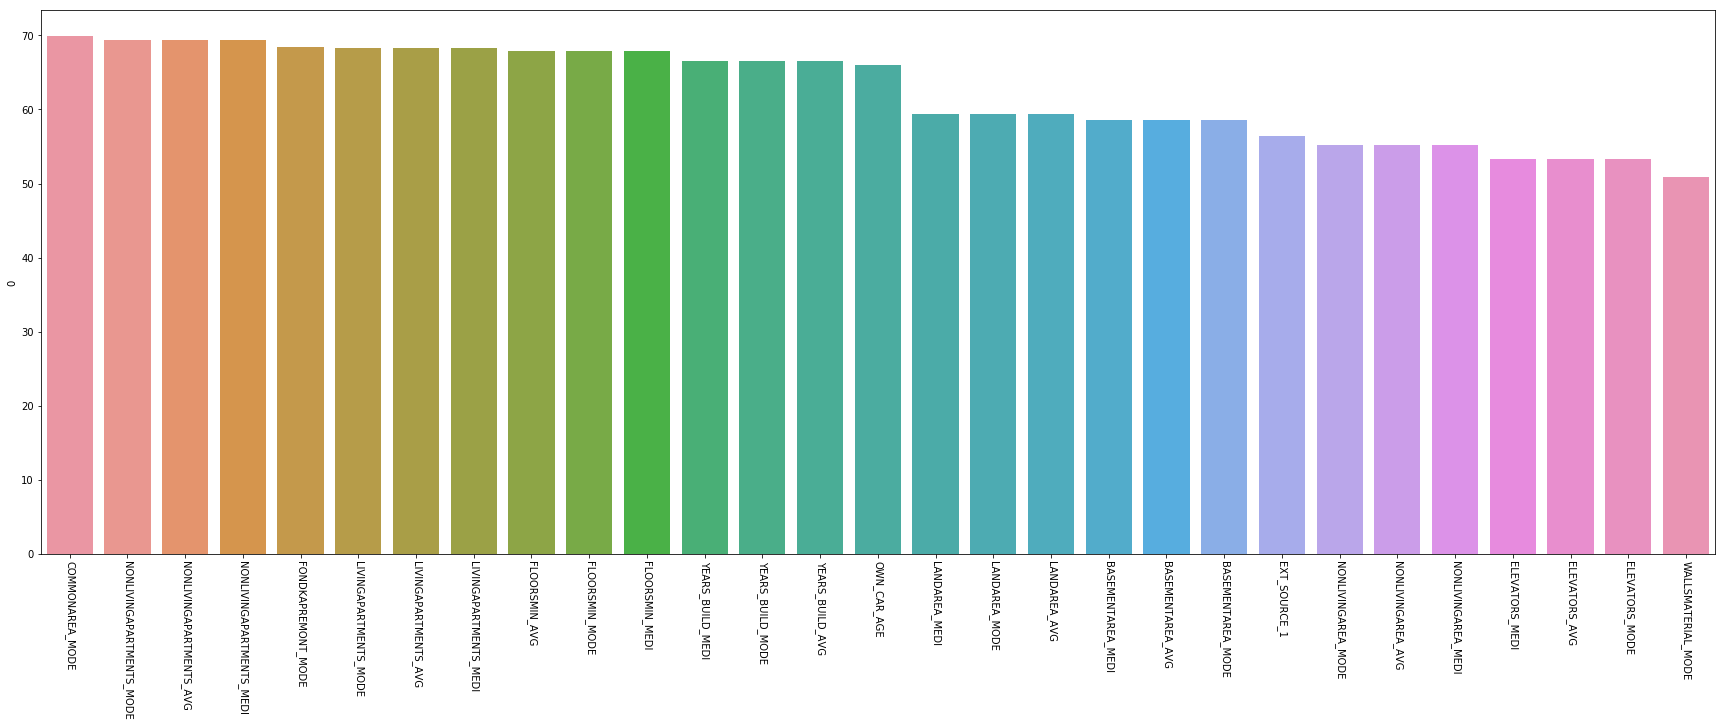
\includegraphics[scale=0.25]{NA2.png}
\caption{Wykres przedstawiający stosunek brakujących wartości w kolumnach $application$}
\end{figure}

\FloatBarrier

Kolumny z ponad połową brakujących wartości zdecydowaliśmy się od razu odrzucić, uznając je za bezużyteczne dla naszego modelu.
Pozostałe braki danych będziemy starali się uzupełnić w kolejnej fazie projektu.

\subsubsection {Pozostałe zbiory}

\begin{table}[h]
\begin{tabular}{lccc}

nazwa zbioru & \% NA & kolumny z NA & kolumny z ponad połową NA \\ 
\hline \hline
bureau                & 13.5 & 7 & 3  \\
bureau\_balance       & 0 & 0 & 0  \\
previous\_application & 18  & 16 & 4 \\
credit\_card          & 6.5  & 9 & 0 \\
installment\_payments & ~0 & 2 & 0 \\
\end{tabular}
\end{table}

\newpage

\subsection{Analiza zależnosci z targetem (application\_train)}

Wykres korelacji zmiennych:


\begin{figure}[h!]
\centering
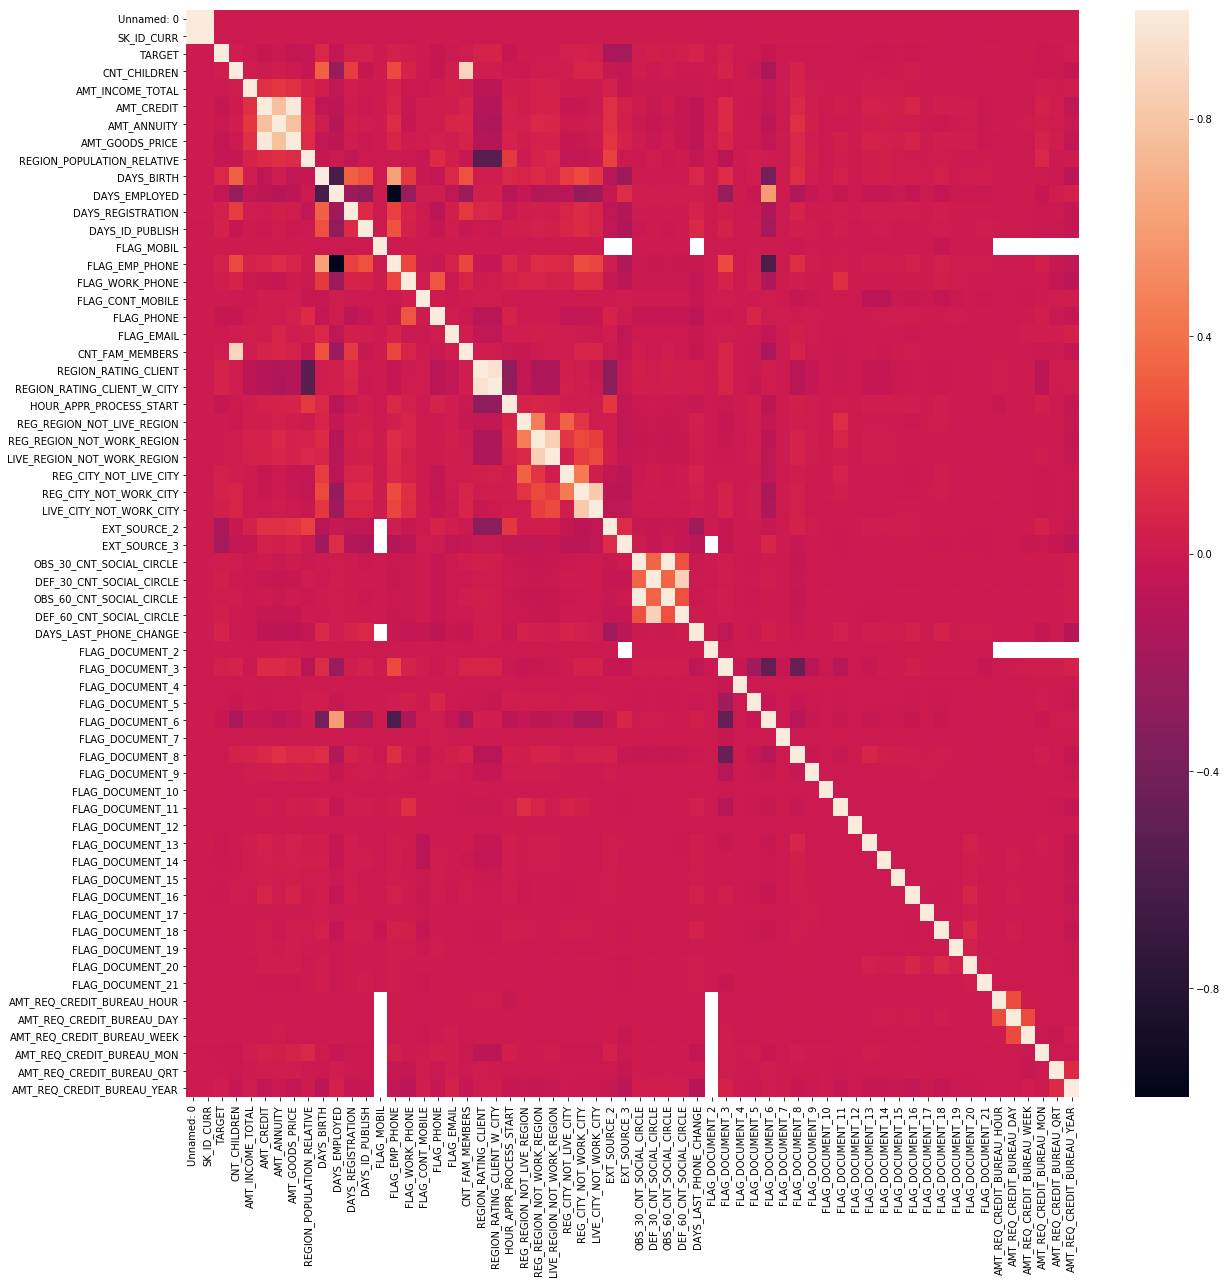
\includegraphics[scale=0.35]{corr.png}
\caption{Wykres korelacji zmiennych w $application$}
\end{figure}


\FloatBarrier

\newpage
\subsubsection{Zależnosci z poszczególnymi zmiennymi kategorycznymi}

Dla poszczególnych zmiennych kategorycznych po lewej stronie przedstawiamy liczności wystąpień poszczególnych kategorii, a po prawej liczności tych kategorii dla TARGETU równego 1.




\begin{figure}[h!]
\centering
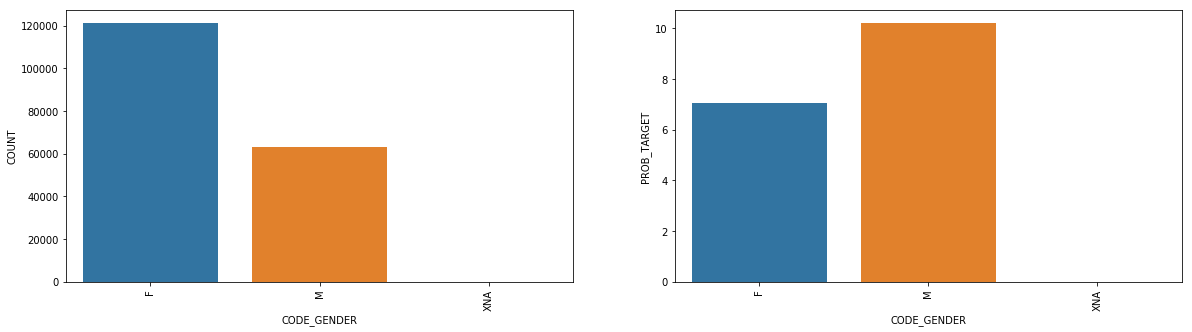
\includegraphics[scale=0.35]{gender.png}
\caption{CODE\_GENDER}
\end{figure}


Zdecydowanie więcej kobiet składało aplikacje kredytowe, ale więcej mężczyzn nie miało problemów ze spłatą kredytu.


\begin{figure}[h!]
\centering
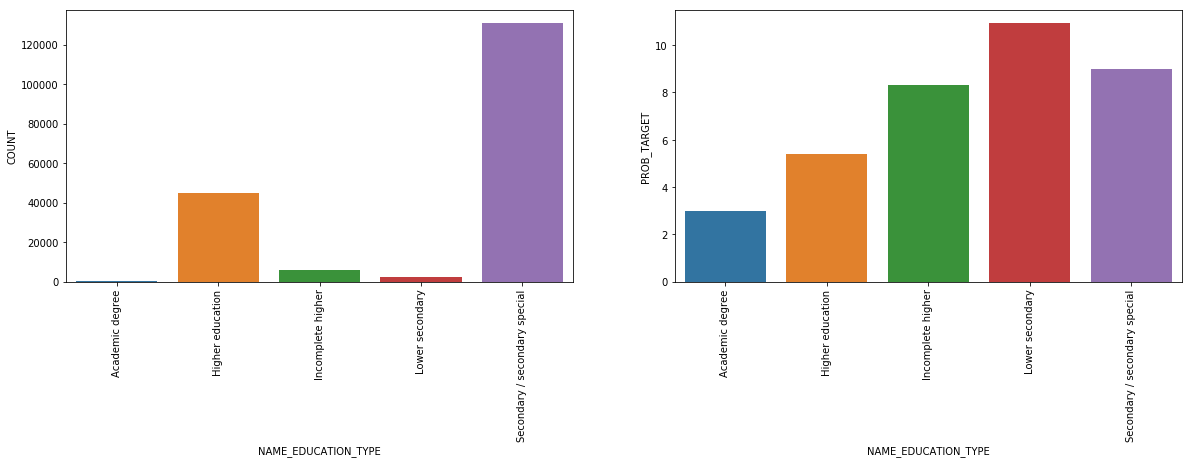
\includegraphics[scale=0.35]{education.png}
\caption{NAME\_EDUCATION\_TYPE}
\end{figure}

Najwięcej aplikacji kredytowych wpłynęło od osób w wykształceniem średnim lub wyższym.

\newpage

\begin{figure}[h!]
\centering
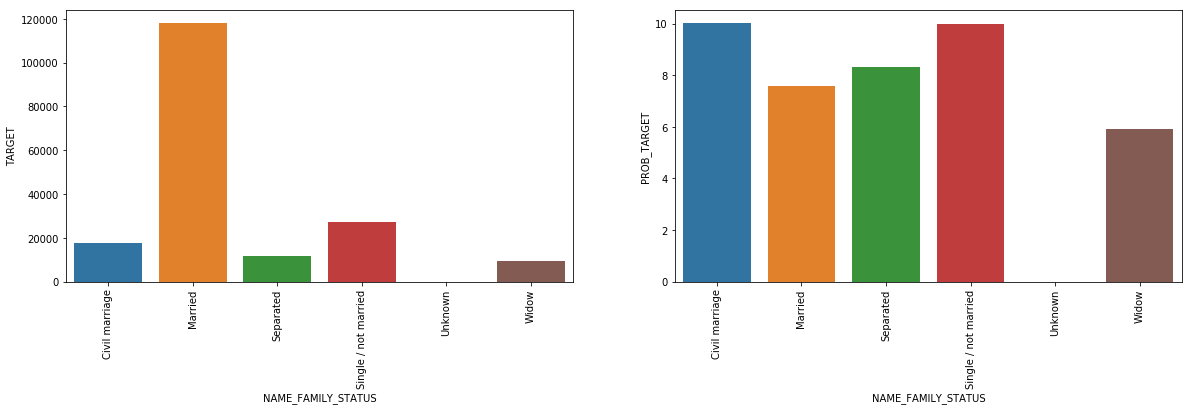
\includegraphics[scale=0.35]{family.png}
\caption{NAME\_FAMILY\_STATUS}
\end{figure}

\newpage
 
\section{Inżynieria cech}

\begin {itemize}
\item {Krok 1 - usunięcie braków danych}

W poprzedniej fazie projektu usunęliśmy już kolumny mające więcej niż 50\% wartości NA. W pozostałych kolumnach chcemy uzupełnić braki danych.
Dla zmiennych numerycznych zdecydowaliśmy się wstawić w miejsca braków danych medianę wartości poszczególnych kolumn.
Dla zmiennych kategorycznych w miejsce wartości NA wstawiamy status "Unknown" - tworzy to odrębną kategorię tej zmiennej.

\item {Krok 2 - EXT-SOURCE}

W zbiorze danych mieliśmy dwie zmienne oznaczające ocenę klienta wydaną przez zewnętrzne źródła: EXT\_SOURCE\_2 i EXT\_SOURCE\_3. Jedna z nich miała dużo brakujących wartości, więc postanowiliśmy uśrednić ich wyniki. Dało nam to nową zmienną, która była lepiej skorelowana ze zmienną TARGET, a~także pozbyliśmy się wielu brakujących wartości.

\item {Krok 3 - ograniczenie się do najważniejszych zmiennych}

Patrząc na korelację poszczególnych kolumn z targetem postanowiliśmy zostawić jedynie kilka najważniejszych zmiennych ze zbioru application\_train:

\begin{itemize}
\item{TARGET} 
\item{SK\_ID\_CURR} 
\item{EXT\_SOURCE} 
\item{DAYS\_BIRTH} 
\item{REGION\_RATING\_CLIENT\_W\_CITY} 
\item{FLAG\_EMP\_PHONE} 
\item{AMT\_GOODS\_PRICE} 
\item{CNT\_CHILDREN} 
\item{FLAG\_DOCUMENT\_3}
\item{CODE\_GENDER}
\end{itemize}

\item {Krok 4 - One Hot Encoding}

Do wszystkich zmiennych kategorycznych zastosowaliśmy One Hot Encoding.

\item {Krok 5 - Przygotowanie i dołączenie danych ze zbioru previous\_application}

W zbiorze $installments\_payments$ dla każdego kredytu mamy informacje o~spłacie kolejnych rat. Na podstawie wymaganych oraz rzeczywistych terminów spłaty rat utworzyliśmy nową kolumnę DAYS\_DELAY (liczba dni opóźnienia w spłacie). Następnie podsumowaliśmy wartości w tej kolumnie dla każdego kredytu - kolumna IS\_DELAYED oznaczająca liczbę opóźnionych spłat kredytu. Dodatkowo powstała kolumna COUNT\_INST oznaczająca łączną liczbę rat kredytu. 

Tak utworzone kolumny dołączyliśmy do zbioru $previous\_application$ (dla odpowiednich SK\_ID\_ PREV). 

W zbiorze $previous\_application$ dokonaliśmy One Hot Encodingu na wszystkich zmiennych kategorycznych, zwiększając tym samym liczbę kolumn do ok. 170.

Aby zbiór danych można było dołączyć do głównego zbioru $application$ zagregowaliśmy dane o tych samych klientach (według SK\_ID\_CURR) za pomocą funkcji sum(). Korzystając z kolumn IS\_DELAYED oraz COUNT\_INST utworzyliśmy kolumnę PERCENT\_DELAY - procent rat kredytów, które były opóźnione w spłacie.

\item {Krok 6 - Przygotowanie i dołączenie danych ze zbioru bureau}

Przygotowanie zbioru $bureau$ sprowadziło się do usunięcia kolumn, w których zawarta była duża liczba brakujących wartości. Wyrzuciliśmy także kolumnę DAYS\_CREDIT\_UPDATE, ponieważ była ona silnie skorelowana z kolumną DAYS\_CREDIT. Taki zbiór dołączyliśmy do naszego bazowego zbioru po kolumnie SK\_ID\_CURR. Ponieważ niewszyscy klienci, którzy znajdowali się w~zbiorze $application$ mieli historię kredytową w $bureau$, to powstało w ten sposób wiele brakujących wartości. Skupiliśmy się więc na klientach, których dane były zawarte w $bureau$, tzn. zostawiliśmy w zbiorze danych te osoby, które pojawił się w zbiorze $bureau$.

\item {Krok 7 - Ostateczne usunięcie braków danych}

Braki danych, które pojawiły się po joinie wszystkich tabel zastąpiliśmy wartością -1.

\end{itemize}

\newpage

\section{Wybór modeli klasyfikacyjnych}

Po zapoznaniu się ze zbiorem danych postanowiliśmy wybrać kilka modeli klasyfikacyjnych do przetestowania.  Postanowiliśmy spojrzeć najpierw na struktury drzewiaste. W naszym przypadku na początku wybraliśmy dwie: \texttt{DecisionTreeClassifier} oraz \texttt{ExtraTreeClassifier}.\\

\begin{figure}[h!]
\centering
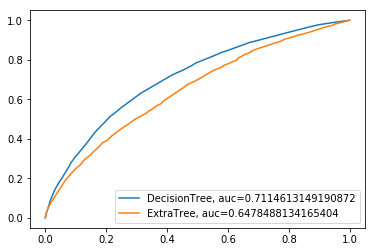
\includegraphics[scale=0.7]{DecisionExtra.png} 
\caption{Wykres AUC DecisionTree i ExtraTree}
\end{figure}

Po wstępnym strojeniu parametrów \texttt{DecisionTree} ma dużo lepsze właściwości predykcyjne niż \texttt{ExtraTree}, więc Jak narazie \texttt{ExtraTree} możemy odrzucić.\\

Następnie spojrzeliśmy na najprostsze modele. Naszą uwagę zwróciła regresja logistyczna. W tym przypadku na domyślnych parametrach uzyskaliśmy AUC rzędu $0.74$, gdzie AUC \texttt{DecisionTree} waha się w okolicach $0.71$.

\begin{figure}[h!]
\centering
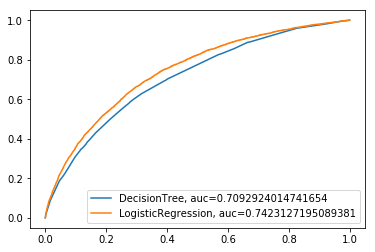
\includegraphics[scale=0.7]{DecisionLogistic.png}
\caption{Wykres AUC DecisionTree i LogisticRegression}
\end{figure}

\newpage

Na koniec przyjrzeliśmy się modelom boostingowym. Wybraliśmy \texttt{LightGBM}, ponieważ dawał on najwyższe AUC podczas testów oraz bardzo szybko się liczył. Na tym etapie odrzuciliśmy \texttt{DecisionTree}, gdyż w \texttt{LightGBM} boosting jest robiony m.in. na drzewach decyzyjnych, więc jeśli drzewa decyzyjne dawałyby najlepsze wyniki to powinno to nam wyjść przy strojeniu parametrów.

\begin{figure}[h!]
\centering
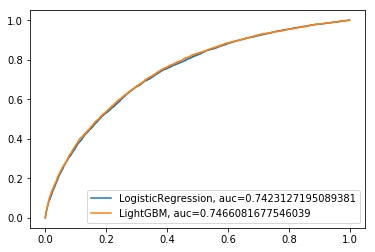
\includegraphics[scale=0.7]{LogisticLGBM.png}
\caption{Wykres AUC LogisticRegression i LightGBM}
\end{figure}

Ponieważ podstawowy model regresji logistycznej nie ma parametrów, to postanowiliśmy, że dokładne strojenie hiperparametrów przeprowadzimy tylko na \texttt{LightGBM}. Rezultaty były gorsze niż się spodziewaliśmy, ponieważ AUC podniosło się jedynie o~około $0.0002$.

\begin{figure}[h!]
\centering
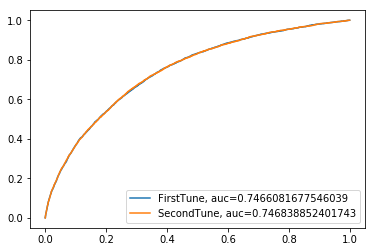
\includegraphics[scale=0.7]{LGBMTuned.png}
\caption{Wykres AUC LightGBM po wstępnym strojeniu hiperparametrów oraz po dokładnym strojeniu}
\end{figure}

\newpage
	
\section{Podsumowanie i wnioski}

Ocena zdolności kredytowej klientów banku to bardzo złożony problem. Mamy tutaj doczynienia z wieloma, często enigmatycznymi, zmiennymi. Pojawia się także wiele brakujących wartości, które trudno w jakiś sposób zastąpić. Staraliśmy się w tym projekcie usuwać jak najmniej informacji. Dzięki takiemu podejściu na końcu uzyskaliśmy prawie 80 zmiennych. W tej sytuacji najlepiej zachowały się struktury drzewiaste oraz regresja liniowa. O ile te pierwsze nie są wcale zaskoczeniem co do swojej skuteczności, o tyle prosty model liniowy uzyskujący wyniki zbliżone do boostingu potrafi być zaskoczeniem dla początkujących analityków danych. LightGBM, który osiągał tutaj najlepsze wyniki nie jest bazowym modelem w bibliotece scikit-learn, a to uczy, że warto spojrzeć na algorytmy, które nie są dołączone w podstawowych wersjach bibliotek. Udało nam się uzyskać AUC w okolicach $0.75$ co jest zbliżone, a jednocześnie dalekie od osiąganych przez specjalistów w tej dziedzinie $0.81$. Na pewno prześledzimy jeszcze wiele razy cały nasz proces tworzenia tego projektu, żeby odnaleźć momenty, w których mogliśmy poprawić nasze AUC, ale i tak jesteśmy zadowoleni oraz dumni z tego co udało nam się uzyskać.


\end{document}